%!TEX root = Main.tex

\section{Simulation} \label{sec:simulation}


\subsection*{Combine subjects}
\begin{enumerate}
\item For each subject, obtain the best permutation in terms of the closest connecting patterns between subjects.
\begin{enumerate}
\item Brute-force search.
\end{enumerate}

\item Combine nodes in the same cluster across subjects, re-estimate  connecting patterns.
\begin{enumerate}
\item Assume the distribution of time shifts are the same across subjects. So when combining subjects, the time shifts do not change. 
\end{enumerate}

\end{enumerate}


\subsection*{Update clustering}
\begin{enumerate}
\item For each node, obtain its connecting pattern with every (permuted) cluster. 
\begin{enumerate}
\item Use the time shifts that produce smaller variance of event times.
\end{enumerate}

\item (Given an estimate of connecting patterns): Assign nodes to the cluster with the most similar connecting patterns.

\item (Given an estimate of clustering): Alternatively, proceed from the first step and compute the pairwise distance matrix, then use spectral clustering.
\end{enumerate}

% \subsection*{Update time shifts?}


\subsection*{Re-clustering result}


\begin{figure}[H]
\includegraphics[width=.6\textwidth]{../simulation/plots/case2_conn_patt}
\caption{(30+30+30). Estimated connecting patterns. Distribution of connecting patterns: $\Gamma(2,0.5),\Gamma(1,0.5),N(0,1)$}
\end{figure}


\begin{figure}[H]
\includegraphics[width=.5\textwidth]{../simulation/plots/case2_cont_cluster}
\caption{Case2 (30+30+30). Combine 5 subjects, and iterate twice.}
\end{figure}


\begin{figure}[H]
\includegraphics[width=.5\textwidth]{../simulation/plots/case3_cont_cluster}
\caption{Case3 (50+50+50). Other settings are the same as above. Combine 5 subjects, and iterate twice.}
\end{figure}



\subsection{Previous results}

\subsection*{Over-clustering can help to reduce the within cluster variability caused by time shifts.}

\begin{figure}[H]
\includegraphics[width=.6\textwidth]{../simulation/plots/case2_conn_patt_matrix}
\caption{Case 2 (50+50+50). Estimated connecting patterns.}
\end{figure}


\begin{figure}[H]
\includegraphics[width=.6\textwidth]{../simulation/plots/case2_overclus_result_boxplot}
\caption{Case 2 (50+50+50). $\tau\sim U(0,10)$. Spectral clustering result with the exact number of clusters vs over-clustering  and merge. 
Five clusters give the best ARI result. Four is not enough, and six makes the clusters too small and hence leads to poor estimation of the connecting patterns.}
\end{figure}

\begin{figure}[H]
\begin{minipage}{0.5\textwidth}
\begin{subfigure}{\textwidth}
\includegraphics[width=\textwidth]{../simulation/plots/case2_exactclus_res}
\caption{Clustering result with k=3. $\triangle$ nodes are clustered into two clusters because of the large variability of time delay parameters.}
\end{subfigure}
\end{minipage}
\begin{minipage}{0.49\textwidth}
\begin{subfigure}{\textwidth}
\includegraphics[width=\textwidth]{../simulation/plots/case2_overclus_res}
\caption{Clustering result with k=5. $\triangle$ nodes are clustered according to time lags. $+$ nodes can be distinguished from $\triangle$'s.}
\end{subfigure}
\begin{subfigure}{\textwidth}
\includegraphics[width=\textwidth]{../simulation/plots/case2_overclusNmerge_res}
\caption{Clustering result after merging similar clusters so that only three clusters are left.}
\end{subfigure}
\end{minipage}
\end{figure}






\subsection*{Non-identifiability}
The second and third clusters are not identifiable.







\subsection*{Over-clustering does not always help}
Possible reasons:
\begin{itemize}
	\item Makes some clusters too small, the estimate for connecting patterns get worse.
	\item Spectral clustering does not keep hierarchical structure, over-clustering may get worse clustering results.
	\item Individual connecting patterns are similar after eliminating  time lags between groups, so different (but similar) groups might be merged together. 
\end{itemize}







\subsection*{Time lag can influence the spatial homogeneity?}

\begin{figure}[H]
\includegraphics[width=.6\textwidth]{../simulation/plots/case1_conn_patt_mat}
\caption{Case 1 (50+50). $\tau\sim U(0,20)$. Estimated connecting patterns. Estimation for the upper left pdf is not good enough because of the time shifts(cannot decide which node dominates the other).}
\end{figure}


\begin{figure}[H]
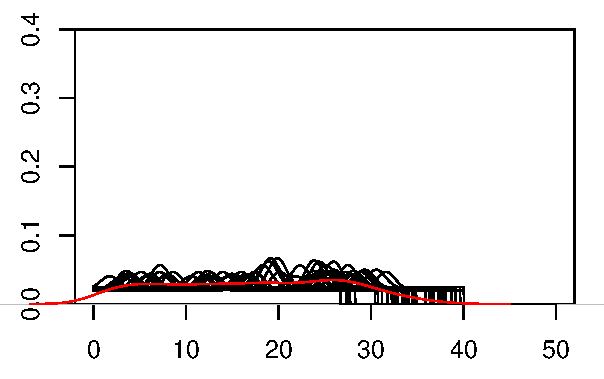
\includegraphics[width=.49\textwidth]{../simulation/plots/case1_clus1}
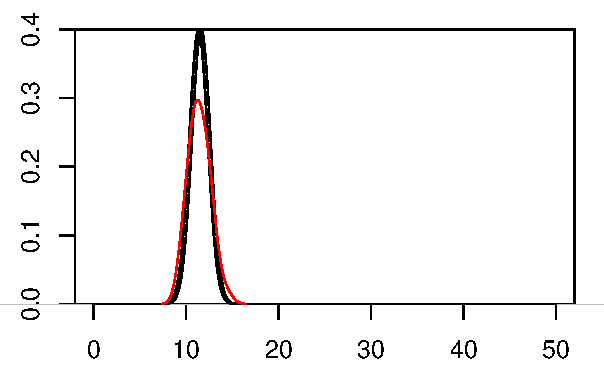
\includegraphics[width=.49\textwidth]{../simulation/plots/case1_clus2}
\caption{Case 1 (50+50). $\tau\sim U(0,20)$. pdf of two clusters.}
\end{figure}


Over-clustering can help provided that the cluster sizes are not too small.

\begin{figure}[H]
\includegraphics[width=.6\textwidth]{../simulation/plots/case1_conn_patt_mat_overclus}
\caption{Case 1 (50+50). $\tau\sim U(0,20)$. Estimated connecting patterns.}
\end{figure}


\begin{figure}[H]
\includegraphics[width=.5\textwidth]{../simulation/plots/case1_clus_res}
\caption{Case 1 (50+50). $\tau\sim U(0,20)$. Clustering result with exact cluster number vs over-clustering and merge.}
\end{figure}







% \subsection*{Remark}
% \begin{enumerate}
% \item Using pdf can avoid getting large distance between curves with similar shapes but different peak heights
% \item Smoothing can cause non-identifiability of uniform distribution and normal distribution.
% \item A bigger size of clusters can lead to a better smooth result.
% \item When combining subjects, consider the biological clock?
% \item Spectral clustering does not keep hierarchical structure.
% \end{enumerate}

In the first case we analyze the network with two types of nodes.
Figure \ref{fig: nodes locations} shows the locations of 50 nodes, among which 4 are from type I and the rest 46 are from type II.
The first type of nodes (type I) are generated uniformly from $[0.3, 0.7]\times[0.8, 5.2]$.
The second type of nodes (type II) are generated uniformly in $[0,1]\times[0,6]$. 
\\

\noindent
The network is developed during time period $[0,50]$.
Two nodes are connected if the distance between them is less than $1$.
The connecting time between two type II nodes is generated from uniform distribution $U(0,40)$.
For the pair of nodes with one from type I and the other from type II, the connecting time is distributed as $N(5+\tau,1)$, where $\tau$ is the time delay caused by the type I node and is generated randomly from $U(0,30)$.

\noindent
Clustering results for one trial are shown in Fig \ref{fig: clustering result, case1}.
\\


% Due to the uncertainty caused by initialization, five independent initializations are used for each trial, and only the one with the largest distance between estimated mean curves is kept.
\noindent
The k-means++ initialization method is performed. 
For each trial, three independent initializations are conducted, and only the one leading to the largest 
between-cluster distance
is kept, where the between-cluster distance is defined as the minimum pairwise distance between estimated mean  functions.
The clustering result is measured using adjusted rand index (ARI), which is also used in \cite{Matias2018}.
The algorithm is tested in 100 synthetic networks. 
The ARI is compared between trials based on c.d.f. and those based on smoothed p.d.f.,
and the result is shown in Figure \ref{fig: ARI, case1}.



The second case is with three clusters.
The locations of nodes are displayed in Figure \ref{fig: nodes locations, case 2}.
The connecting radius for type I node is set as $2$, and that for other nodes is set as $1$. 
For a pair of type III nodes, the connecting time is generated from uniform distribution $U(0,30)$.
For the pair of nodes with one from type II and the other from type III, 
the connecting time is distributed as $N(5+\tau,1)$, where $\tau$ is the time delay caused by the type II node and is generated randomly from $U(0,5)$.
For the pair of nodes with one from type I and the other from type II, the connecting time is distributed as $U(\tau,\tau+6)$, where $\tau$ is the time delay caused by the type II node and is generated randomly from $U(40,42)$.



\noindent
Clustering results for one trial are shown in Fig \ref{fig: clustering result, case2}.
\\


\noindent
100 independent trials are recorded. 
The k-means++ initialization is applied for each trial.
The ARI is displayed in Figure \ref{fig: ARI, case2}.



The third case has similar set up as Case 2, except that 
the time delays of the type II nodes are generated from $U(0,30)$ (it was $U(0,5)$ in the second case).

\noindent
Clustering results for one trial are shown in Fig \ref{fig: clustering result, case3}.
\\


\noindent
100 independent trials are recorded. 
The k-means++ initialization is applied for each trial.
The ARI is displayed in Figure \ref{fig: ARI, case3}.




